\documentclass[12pt, letterpaper]{report}
\usepackage[a4paper, margin=0.7in, top=20mm, bottom=20mm]{geometry}
\usepackage{mathspec}
\usepackage[UTF8]{ctex}
\usepackage[colorlinks=true, linkcolor=black, urlcolor=blue]{hyperref}
\usepackage{listings}
\usepackage{xcolor}
\usepackage{graphicx}
\usepackage{xparse}
\usepackage{tcolorbox}
\usepackage{mdframed}

\graphicspath{ {./pics/} }

% ---- Code Section Style ----
\colorlet{mygray}{black!30}
\colorlet{mygreen}{green!60!blue}
\colorlet{mymauve}{red!60!blue}

\tcbuselibrary{breakable}
\NewDocumentCommand{\exercise}{ m +m }{
    {
        \edef\originalParIndent{\the\parindent}
        \begin{tcolorbox}[breakable,arc=0mm,boxrule=0.8pt]
            \setlength{\parindent}{\originalParIndent}
            \noindent
            \textbf{\large Exercise #1}
            \indent
            #2
        \end{tcolorbox}
    }
}

\tcbuselibrary{breakable}
\NewDocumentCommand{\question}{ m +m }{
    {
        \edef\originalParIndent{\the\parindent}
        \begin{tcolorbox}[breakable,arc=0mm,boxrule=0.8pt]
            \setlength{\parindent}{\originalParIndent}
            \noindent
            \textbf{\large Question}
            \indent
            #2
        \end{tcolorbox}
    }
}

\lstdefinelanguage
   [x64]{Assembler}     % add a "x64" dialect of Assembler
   [x86masm]{Assembler} % based on the "x86masm" dialect
   % with these extra keywords:
   {morekeywords={CDQE,CQO,CMPSQ,CMPXCHG16B,JRCXZ,LODSQ,MOVSXD, %
                  POPFQ,PUSHFQ,SCASQ,STOSQ,IRETQ,RDTSCP,SWAPGS, %
                  rax,rdx,rcx,rbx,rsi,rdi,rsp,rbp, %
                  r8,r8d,r8w,r8b,r9,r9d,r9w,r9b, %
                  r10,r10d,r10w,r10b,r11,r11d,r11w,r11b, %
                  r12,r12d,r12w,r12b,r13,r13d,r13w,r13b, %
                  r14,r14d,r14w,r14b,r15,r15d,r15w,r15b}} % etc.


\lstset{
  backgroundcolor=\color{gray!10},  
  basicstyle=\ttfamily,
  columns=fullflexible,
  breakatwhitespace=false,      
  breaklines=true,                
  captionpos=b,                    
  commentstyle=\color{mygreen}, 
  extendedchars=true,              
  frame=single,                   
  keepspaces=true,             
  keywordstyle=\color{blue},                    
  numbers=none,                
  numbersep=5pt,                   
  numberstyle=\tiny\color{blue}, 
  rulecolor=\color{mygray},        
  showspaces=false,               
  showtabs=false,                 
  stepnumber=5,                  
  stringstyle=\color{mymauve},    
  tabsize=3,                      
  title=\lstname                
}

\lstdefinestyle{CStyle}{  
    % commentstyle=\color{mGreen},
    % keywordstyle=\color{magenta},
    % numberstyle=\tiny\color{mGray},
    % stringstyle=\color{mPurple},
    basicstyle=\footnotesize,
    breakatwhitespace=false,                              
    showstringspaces=false,
    language=C
}

\lstdefinestyle{AssemblyStyle}{  
    basicstyle=\footnotesize,
    breakatwhitespace=false,                              
    showstringspaces=false,
    language=[x64] Assembler
}


\lstdefinestyle{MakeFileStyle}{  
    basicstyle=\footnotesize,
    breakatwhitespace=false,                              
    showstringspaces=false,
    language=[gnu] make
}


% ----------------------------


\setcounter{chapter}{0}
\setlength{\parindent}{2em}
\setmainfont{Times New Roman}
\setcounter{tocdepth}{1}
\setcounter{secnumdepth}{1}

\title{MIT6.828 Lab2: Memory Management}
\author{Zhuofan Zhang}
\date{Jan 2022}



\begin{document}
\maketitle
% ---- Contents ----
\pagenumbering{roman}
\renewcommand\contentsname{\Huge Contents}
\tableofcontents{}
% ------------------


% ---- Part A ---------------------------------
\newpage
\pagenumbering{arabic}
\chapter[\Large Physical Page Management]{Physical Page Management}
本次 Lab 的内容主要分为两个部分,第一个部分是对可用物理内存的管理,第二个部分是虚拟内存的管理。\par
操作系统负责对可用物理内存的管理。JOS 的物理页使用 PageInfo 结构相关数据(数组/空闲链表)进行物理内存管理。
PageInfo 数组(pages)是对整个物理地址空间中可用内存(base-mem + extend-mem)的映射:将整个物理地址空间按4KB-page划分,则每个单页
可由pages对应下标的 PageInfo 结构唯一指代(原理可见 pmap.h/page2pa 的实现)。\par
下图为xv6的VA-PA映射关系图,在本次 Lab 中我们将在 JOS 上实现类似的映射。 
\quad \par 
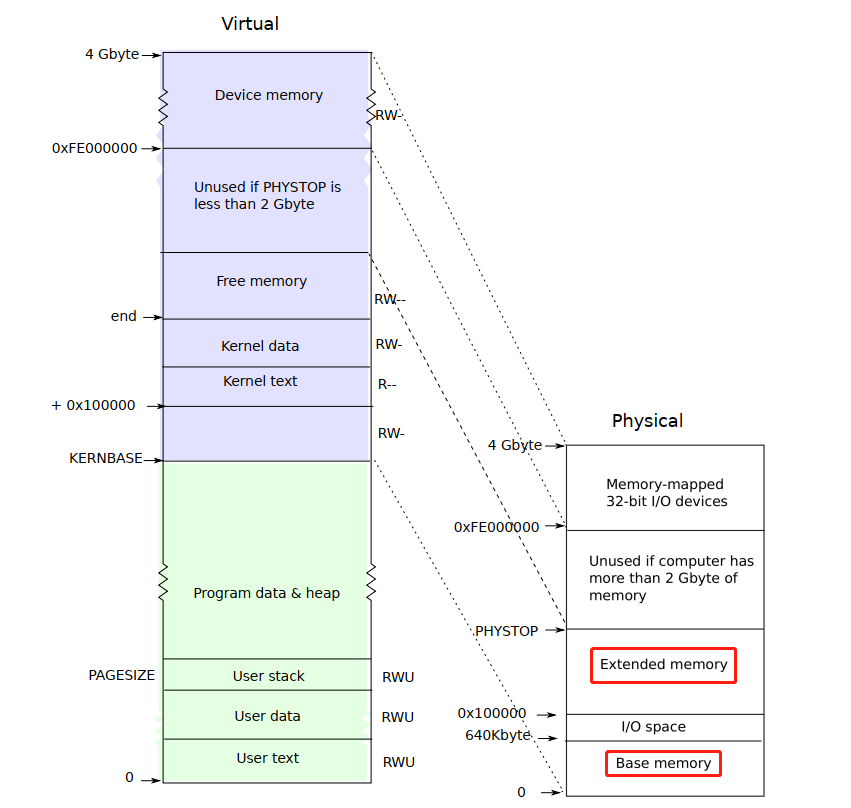
\includegraphics[width=0.8\textwidth]{layout-of-vapa}
\newpage
\exercise{1}{
        \par 
        \noindent {In the file kern/pmap.c, you must implement code 
        for the following functions:}
        \quad \par 
        \noindent \textbf{boot\_alloc() } \par
        \noindent \textbf{mem\_init() (only up to the call to check\_page\_free\_list(1))} \par
        \noindent \textbf{page\_init()} \par
        \noindent \textbf{page\_alloc()} \par
        \noindent \textbf{page\_free()} \par
        \quad \par 
        \noindent {check\_page\_free\_list() and check\_page\_alloc() test your physical page
        allocator. You should boot JOS and see whether check\_page\_alloc() reports success. 
        Fix your code so that it passes. You may find it helpful to add your own assert()s 
        to verify that your assumptions are correct.} \par
}
根据题目要求,我们依次实现上述函数。\par 
对于 \textbf{boot\_alloc} 函数,根据注释提示可知其为系统启动初期的 physical-page allocator,协助完成初始化工作。
函数中使用了一个变量 end,我们从内核的链接脚本(kernel.ld)中可以定位到它的位置,即.BSS段的末尾;根据注释提示,
end 表示第一处未被 kernel 使用的\underline{虚拟地址}。由 Lab1 可知内核被链接至高地址位(0xf0100000开始的4MB区域),
因此也许保证在这个阶段分配的物理内存不超过4MB,需要对分配是否越界进行检查。明确上述要求后,我们即可实现该函数:
% \newpage

\lstset{style=CStyle}
\setmainfont{Consolas}
\begin{lstlisting}
static void *
boot_alloc(uint32_t n)
{
    ...

    // Allocate a chunk large enough to hold 'n' bytes, then update
    // nextfree.  Make sure nextfree is kept aligned
    // to a multiple of PGSIZE.
    //
    // LAB 2: Your code here.
    result = nextfree;
    if(n > 0)
        nextfree = ROUNDUP(nextfree + n, PGSIZE);
    else if(n < 0)
        // n < 0: should not come here
        panic("boot_alloc: parameter n < 0.");

    if(PADDR(nextfree) >= 0x400000)
        panic("boot_alloc: run out of mem.");
    return result;
}
\end{lstlisting}
\setmainfont{Times New Roman}
\quad \par

\textbf{mem\_init} 函数是被内核 i386\_init() 调用的函数,用来完成内核内存管理的初始化;
本节仅需完成物理内存管理相关的部分。\par 
根据本节开头我们提到的物理内存管理方法,我们首先需要创建管理物理页的数组pages。由于pages本身也需要
占用内存,我们利用上一步实现的 boot\_alloc 分配内存并将pages进行0初始化。需要注意的是数组大小(npages)由 
i386\_detect\_memory 调用得到,它负责检查系统可用的物理内存大小。根据上述分析,我们实现 mem\_init 中初始化
pages部分的内容:\par 

\lstset{style=CStyle}
\setmainfont{Consolas}
\begin{lstlisting}
void
mem_init(void)
{
    ...

    // Find out how much memory the machine has (npages & npages_basemem).
    i386_detect_memory();

    ...

    //////////////////////////////////////////////////////////////////////
    // Allocate an array of npages 'struct PageInfo's and store it in 'pages'.
    // The kernel uses this array to keep track of physical pages: for
    // each physical page, there is a corresponding struct PageInfo in this
    // array.  'npages' is the number of physical pages in memory.  Use memset
    // to initialize all fields of each struct PageInfo to 0.
    // Your code goes here:
    pages = (struct PageInfo *) boot_alloc(npages * sizeof(struct PageInfo));
    memset(pages, 0, npages * sizeof(struct PageInfo));

    ...
}
\end{lstlisting}
\setmainfont{Times New Roman}
\quad \par

上一步实现的代码中,我们可以看到在为pages分配内存并进行0初始化后,mem\_init 调用了真正
对pages及空闲列表page\_free\_list进行初始化的 \textbf{page\_init} 。
根据 Lab1 中提到的 PC's Physical Address Space 的布局我们可知,物理空间中可用内存
由 Base-memory 和 Extended-memory 两部分组成,我们需要将这些可用的内存放入空闲链表;
由于实际上系统运行至这一步时已经使用了一部分物理页,这部分页不应再放入空闲列表;
此外,物理空间中也存在一些不可使用的段(IO holes/BIOS/...),我们也许将其排除。\par
根据 page\_init 中的提示,我们完成代码如下。
其中比较需要关注的是 extended memory 空闲部分的初始化,第三步除了设置IO hole不空闲外,也需设置已经被使用的物理页,
而确定当前已用物理页位置末端(以虚拟地址表示)的方法是对 boot\_alloc 的零调用:\par 

\newpage
\lstset{style=CStyle}
\setmainfont{Consolas}
\begin{lstlisting}
void
page_init(void)
{
    // The example code here marks all physical pages as free.
    // However this is not truly the case.  What memory is free?
    //  1) Mark physical page 0 as in use.
    //     This way we preserve the real-mode IDT and BIOS structures
    //     in case we ever need them.  (Currently we don't, but...)
    //  2) The rest of base memory, [PGSIZE, npages_basemem * PGSIZE)
    //     is free.
    //  3) Then comes the IO hole [IOPHYSMEM, EXTPHYSMEM), which must
    //     never be allocated.
    //  4) Then extended memory [EXTPHYSMEM, ...).
    //     Some of it is in use, some is free. Where is the kernel
    //     in physical memory?  Which pages are already in use for
    //     page tables and other data structures?
    //
    // Change the code to reflect this.
    // NB: DO NOT actually touch the physical memory corresponding to
    // free pages!
    // 1) Mark physical page 0 as in use
    pages[0].pp_ref = 1;
    // 2) Base-memory
    size_t i;
    for (i = 1; i < npages_basemem; i++) {
        pages[i].pp_ref = 0;
        pages[i].pp_link = page_free_list;
        page_free_list = &pages[i];
    }
    // 3) IO hole + pages that have been used
    int hole_and_used = npages_basemem + 
                        ((EXTPHYSMEM - IOPHYSMEM) + 
                        PADDR(boot_alloc(0)))/PGSIZE;
    for(; i < hole_and_used; i++)
        pages[i].pp_ref = 1;

    // 4) extended memory
    for(; i < npages; i++)
    {
        pages[i].pp_ref = 0;
        pages[i].pp_link = page_free_list;
        page_free_list = &pages[i];
    }
}
\end{lstlisting}
\setmainfont{Times New Roman}
\quad \par

初始化pages及page\_free\_list后,就可以进一步实现分配和回收页的函数:
\textbf{page\_alloc} 与 \textbf{page\_free} 。注意到实现物理页分配时,对页面进行初始化时
\underline{需要获得物理页的虚拟地址}(C语言中地址均匀虚拟地址),
根据提示使用 page2kva 实现。page2kva 本身的实现是使用 page2pa 得到物理页的实际地址,再根据当前
的映射使用 KADDR 转化为虚拟地址。
\lstset{style=CStyle}
\setmainfont{Consolas}
\begin{lstlisting}
struct PageInfo *
page_alloc(int alloc_flags)
{
    // Fill this function in
    if(!page_free_list)
        return NULL;

    struct PageInfo *alloc_page = page_free_list;
    page_free_list = page_free_list->pp_link;
    alloc_page->pp_link = NULL;

    if(alloc_flags & ALLOC_ZERO)
        memset(page2kva(alloc_page), 0, PGSIZE);

    return alloc_page;
}

void
page_free(struct PageInfo *pp)
{
	// Fill this function in
	// Hint: You may want to panic if pp->pp_ref is nonzero or
	// pp->pp_link is not NULL.
	if(pp->pp_ref != 0 || pp->pp_link != NULL)
		panic("page_free: pp_ref != 0");
	
	pp->pp_link = page_free_list;
	page_free_list = pp;

}
\end{lstlisting}
\setmainfont{Times New Roman}

% ------------------------------------------------------------

\chapter[\Large Virtual Memory]{Virtual Memory}

\exercise{2}{
        \par 
        \noindent{
            Look at chapters 5 and 6 of the Intel 80386 Reference Manual, 
            if you haven't done so already. Read the sections about page translation 
            and page-based protection closely (5.2 and 6.4). 
            We recommend that you also skim the sections about segmentation; 
            while JOS uses the paging hardware for virtual memory and protection, 
            segment translation and segment-based protection cannot be disabled on the x86, 
            so you will need a basic understanding of it.} \par 
}
\quad \par 
这一节内容需要我们构建虚拟内存管理的基本设施,Exercise2为我们提供了80386处理器内存管理模式的相关材料。
阅读相关材料后,我们可以整理出处理器为我们提供的内存管理机制:分段/分页。

\section[\large Virtual, Linear, and Physical Addresses]{Virtual, Linear, and Physical Addresses}
在x86体系中,我们可以定义3种地址:虚拟地址(Virtual Address, VA)[也称Logical Address],
线性地址(Linear Address, LA)与物理地址(Physical Address, PA)。\par
对于用户而言,可见的只有VA,而数据在物理内存中的实际地址是PA。x86的典型地址翻译流程如下图所示,
其中VA $\rightarrow$ LA 的过程为 \textsl{分段(Segmentation)} 机制,LA $\rightarrow$ PA 过程为 \textsl{分页(Paging)} 机制。\par
关于分页与分段的详细内容不在此处展开,但需知道:JOS 并不使用分段机制,但x86系统并没有显式关闭分段的方法。因此,
在设置 Segment Descript Table 时,JOS 将段基址设置为0,并将 LIMIT 设置为 0xffffffff,即将整个物理地址空间视为
一段,在这种情况下VA = LA。设置的过程在 Lab1 中的 boot 阶段完成(boot.S)。\par 
{
\centering
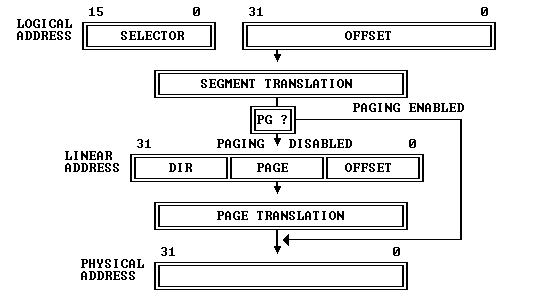
\includegraphics[width=0.8\textwidth]{AddressTranslationOverview}
}
\quad \par 
\quad \par 
\exercise{3}{
        \par 
        \quad {
            While GDB can only access QEMU's memory by virtual address, 
            it's often useful to be able to inspect physical memory 
            while setting up virtual memory. 
            Review the QEMU monitor commands from the lab tools guide, 
            especially the xp command, which lets you inspect physical memory. 
            \underline{To access the QEMU monitor, press Ctrl-a c in the terminal} 
            (the same binding returns to the serial console).
        } \par

        \quad {
            Use the \textbf{xp} command in the QEMU monitor and the x command in GDB 
            to inspect memory at corresponding physical and virtual addresses 
            and make sure you see the same data.
        } \par

        \quad {
            Our patched version of QEMU provides an \textbf{info pg} command that may also prove useful: 
            it shows a compact but detailed representation of the current page tables, 
            including all mapped memory ranges, permissions, and flags. 
            Stock QEMU also provides an \textbf{info mem} command that shows an overview 
            of which ranges of virtual addresses are mapped and with what permissions.
        } \par 
}
\quad \par
这一个练习的第一个要求与 Lab1 类似,要求我们观察虚拟地址与其实际映射到的物理地址的内容是否一致
(即虚拟内存映射是否成功)。与 Lab1 不同,此处采用更泛用的方法:使用GDB观察VA,使用QEMU-monitor观察
PA。根据提示,我们在gdb设置内存映射成功后的位置检查,可以看到VA及其对应的PA内容的一致性:\par 

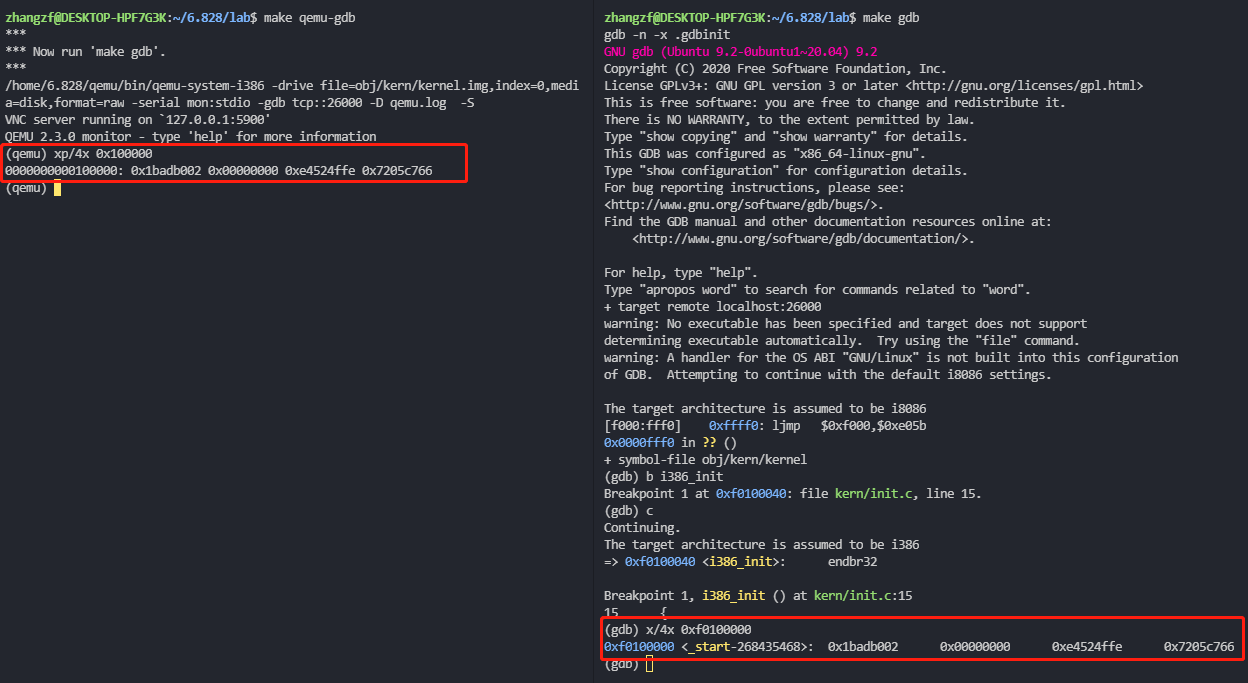
\includegraphics[width=0.85\textwidth]{pa_va}

\quad \par 
此外,我们还根据提示,使用 \textbf{info pg/mem} 命令查看页表情况与内存权限情况:\par 
\quad \par 

\lstset{style=AssemblyStyle}
\setmainfont{Consolas}
\begin{lstlisting}
(qemu) info pg
VPN range     Entry         Flags        Physical page
[00000-003ff]  PDE[000]     ----A----P
    [00000-000ff]  PTE[000-0ff] --------WP 00000-000ff
    [00100-00100]  PTE[100]     ----A---WP 00100
    [00101-00111]  PTE[101-111] --------WP 00101-00111
    [00112-00112]  PTE[112]     ---DA---WP 00112
    [00113-003ff]  PTE[113-3ff] --------WP 00113-003ff
[f0000-f03ff]  PDE[3c0]     ----A---WP
    [f0000-f00ff]  PTE[000-0ff] --------WP 00000-000ff
    [f0100-f0100]  PTE[100]     ----A---WP 00100
    [f0101-f0111]  PTE[101-111] --------WP 00101-00111
    [f0112-f0112]  PTE[112]     ---DA---WP 00112
    [f0113-f03ff]  PTE[113-3ff] --------WP 00113-003ff
(qemu) info mem
0000000000000000-0000000000400000 0000000000400000 -r-
00000000f0000000-00000000f0400000 0000000000400000 -rw
\end{lstlisting}
\setmainfont{Times New Roman}
\quad \par

本节的最后,Lab 还简要介绍了 JOS 中地址类型的 typedef。JOS 将地址类型区分为
虚拟地址(uintptr\_t)与物理地址(physaddr\_t),它们均为 uint32\_t 的typedef。
由于C中所有出现的“地址”均为虚拟地址,故其中uintptr\_t可以被解引用使用,而physaddr\_t
不应被解引用,它仅作为物理地址字面值被使用,对其解引用将引发UB。\par 

\newpage
\section[\large Page Table Management]{Page Table Management}
本节的内容是构建页表管理的API,为下一节构建内核VA映射提供支持。\par 
\quad \par 
\exercise{4}{
    \par 
    \noindent {
        In the file kern/pmap.c, 
        you must implement code for the following functions.
    }
    \quad \par 
    \noindent \textbf{pgdir\_walk() } \par
    \noindent \textbf{boot\_map\_region()} \par
    \noindent \textbf{page\_lookup()} \par
    \noindent \textbf{page\_remove()} \par
    \noindent \textbf{page\_insert()} \par
    \quad \par 
    \noindent {
        check\_page(), called from mem\_init(), 
        tests your page table management routines. 
        You should make sure it reports success before proceeding.
    } \par
}

\subsection{\large pgdir\_walk}
pgdir\_walk 函数的功能是在页表目录(pgdir)查询目标虚拟地址 va,返回指向查询的虚拟地址
对应页表项(PTE)的\underline{指针};若页表项不存在(即 PDE 中 PTE\_P 非置位,对应\underline{页表}不存在),
可以设置 create 选项决定是否创建页表。理解这个函数的实现有两个比较重要的点:\par 
1. 返回的指向对应PTE的指针是什么。我们需要取的是 \underline{va 对应页表的虚拟地址}。
根据 va 对应的 PDE,我们可以得到页表的物理地址(PTE\_ADDR(pde));而根据 Lab1 及前文所述,
\underline{JOS/xv6 都将物理地址空间映射到了高位虚拟地址空间}(即 KERNBASE 上方,见前文 xv6: VA-PA映射图),
因此我们可以通过直接将物理地址加上 KERNBASE(JOS提供了宏:KADDR)得到 pte 的虚拟地址。\par 
\noindent(注:可能存在疑问——当前程序状态仅在虚拟内存空间中映射[0, 4MB)的物理地址,但实际此处分配
得到的页表可能在更高的地址中,是否存在问题?答案是否定的,因为此时我们所有的操作仍未加载到处理器上,
实际该页表目录是等到完整映射构建后才被加载的,当时物理地址空间已被完整映射到JOS-VA的remappad区域。见
Kernel Address Space 一节)\par
2. 若需 create,实际创建了什么。根据Lab-Hints,pgdir\_walk 发生分配时实际上是分配 va 所在的页表,
只需PTE被建立即可,而\underline{ va 实际对应的物理空间仍未被分配}。\par 
根据上述分析,我们可以实现函数如下:\par 
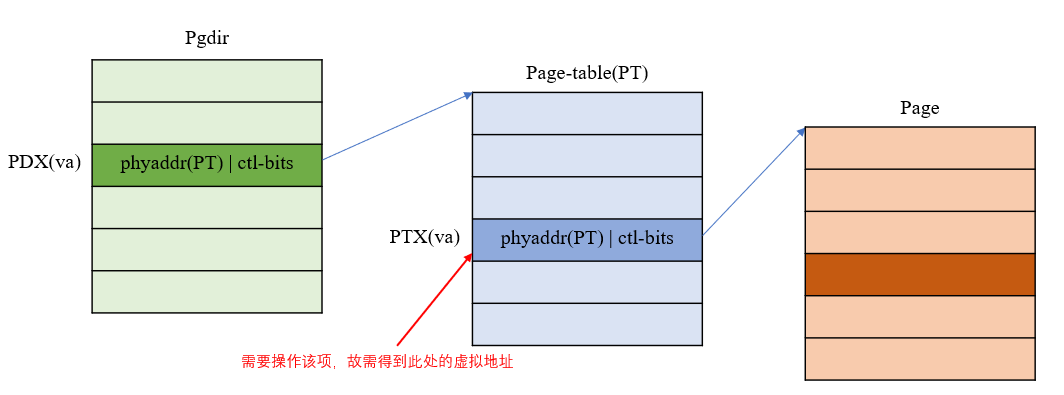
\includegraphics[width=0.8\textwidth]{pgdirwalk}
\lstset{style=CStyle}
\setmainfont{Consolas}
\begin{lstlisting}
pte_t *
pgdir_walk(pde_t *pgdir, const void *va, int create)
{
    // ppde/ppte: point-to-pde/pte
    pde_t *ppde = pgdir + PDX(va); // pde is the VA of pgdir[PDX(va)]
    pte_t *ppte = NULL;			  // default result: NULL
    if(!(*ppde & PTE_P))
    {
        if(create)
        {
            struct PageInfo *new_pt = page_alloc(ALLOC_ZERO);
            if(!new_pt)
                // alloc failed
                return NULL;
            (new_pt->pp_ref)++;
            *ppde = (page2pa(new_pt) | PTE_P | PTE_W | PTE_U);
        }
        else
            return NULL;
    }

    // Don't forget the (pte_t*) cast
    ppte = (pte_t*)KADDR(PTE_ADDR(*ppde)) + PTX(va);	// key: the use of KADDR
    return ppte;
}
\end{lstlisting}
\setmainfont{Times New Roman}


\newpage
\subsection{\large boot\_map\_region}
这个函数是用于构建 PA-VA 的核心函数,用于将 [pa, pa+size) 映射到 [va, va+size)。
Lab-Hints 提示使用 pgdir\_walk 实现,实现结果如下:\par 
\lstset{style=CStyle}
\setmainfont{Consolas}
\begin{lstlisting}
static void
boot_map_region(pde_t *pgdir, uintptr_t va, size_t size, physaddr_t pa, int perm)
{
    if((size % PGSIZE))
    {
        cprintf("HERE:%#x, SIZE:%#x\n", va, size);
        panic("boot_map_region: size is not a multiple of PGSIZE.");
    }

    for(int sz = 0; sz < size; sz += PGSIZE)
    {
        pte_t *pte = pgdir_walk(pgdir, (void *)(va + sz), 1);
        *pte = (pa + sz) | perm | PTE_P;
    }

}
\end{lstlisting}
\setmainfont{Times New Roman}

\subsection{\large page\_lookup}
这个函数用于查找 va 对应的实际物理页(注意与 pgdir\_walk 功能区分),
返回物理页对应的 PageInfo 对象,并可选地记录 PTE 的虚拟地址。若 va 对应的物理页
尚未分配则返回空指针。函数实现如下:\par 
\lstset{style=CStyle}
\setmainfont{Consolas}
\begin{lstlisting}
struct PageInfo *
page_lookup(pde_t *pgdir, void *va, pte_t **pte_store)
{
    // ppte: point-to-pte
    pte_t *ppte = pgdir_walk(pgdir, va, 0);
    if(!ppte)
        return NULL;

    if(!(*ppte & PTE_P))
        return NULL;

    if(pte_store != NULL)
        *pte_store = ppte;

    return pa2page(PTE_ADDR(*ppte));
}
\end{lstlisting}
\setmainfont{Times New Roman}

\newpage

\subsection{\large page\_remove \& page\_insert}
这两个函数用于映射的删除与分配。其中有以下几点需要注意:\par
1. page\_remove 在删除映射时需同时刷新TLB,并在 pp\_ref 引用为0(即页已结束生命期)时
将其重新维护入空闲列表。\par 
2. page\_insert 的 corner\_case。由于实际插入页可能涉及自身替换问题,需先
增加 pp\_ref 再进行旧页 remove 操作,防止错误释放目标页。\par
\quad \par 
\noindent 根据分析后实现代码如下:\par 
\lstset{style=CStyle}
\setmainfont{Consolas}
\begin{lstlisting}
void
page_remove(pde_t *pgdir, void *va)
{
    pte_t *ppte;
    struct PageInfo* unmap_pg = page_lookup(pgdir, va, &ppte);

    // such physic-page exist
    if(unmap_pg)
    {
        *ppte = 0;
        page_decref(unmap_pg);
        tlb_invalidate(pgdir, va);
    }
}

int
page_insert(pde_t *pgdir, struct PageInfo *pp, void *va, int perm)
{
	pte_t *ppte = pgdir_walk(pgdir, va, 1);
	if(!ppte)
		return -E_NO_MEM;
	// Consider the corner-case
	pp->pp_ref++;
	page_remove(pgdir, va);	// If page-map exists, remove it
	*ppte = page2pa(pp) | perm | PTE_P;
	return 0;
}
\end{lstlisting}
\setmainfont{Times New Roman}

% ------------------------------------------------------------

\chapter[\Large Kernel Address Space]{Kernel Address Space}
利用上一章节构建的 API,我们就可以实现 JOS 的内核部分地址空间的映射了。\par 
JOS 的 VAS 布局可以参考 memlayout.h 文件。JOS 将整个地址空间划分为两部分,以 ULIM 为界
下方为用户地址空间,上方为内核地址空间,且 [UTOP, ULIM) 段一经初始化即为只读(内核/用户态均仅有此权限),
是内核为用户态提供的信息。\par 
\quad \par 
\exercise{5}{
        \par 
        \noindent{
            Fill in the missing code in \textbf{mem\_init()} after the call to check\_page().
        } \par 
        \noindent{
            Your code should now pass the \textbf{check\_kern\_pgdir()} and 
            \textbf{check\_page\_installed\_pgdir()} checks.
        } \par 
}
\quad \par 
查看 mem\_init 的 Lab-hints,可以发现我们需要映射内核地址空间的三个部分:
RO PAGES,KERNEL STACK,remapped physical address。根据提示我们即可补全上述代码
完成映射。需要注意的是其中内核栈的顶部设置了一个无效区段,用于限制栈大小并使栈溢出时
产生异常。(注:无效 = 此处的映射无需构建)。\par 
此外,映射时需注意 PTE 的控制位设置,详情可见 Exercise 2 中提供的参考材料。\par
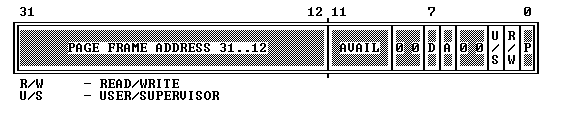
\includegraphics[width=0.8\textwidth]{PTE}
\quad \par 
\noindent 根据分析后实现代码如下:\par 
\lstset{style=CStyle}
\setmainfont{Consolas}
\begin{lstlisting}
boot_map_region(kern_pgdir, UPAGES, PTSIZE, PADDR(pages), PTE_U);
boot_map_region(
    kern_pgdir, KSTACKTOP-KSTKSIZE, KSTKSIZE, 
    PADDR(bootstacktop)-KSTKSIZE, PTE_W
);
boot_map_region(kern_pgdir, KERNBASE, (size_t)(0x40000000000 - KERNBASE), 0, PTE_W);
\end{lstlisting}
\setmainfont{Times New Roman}

\newpage
\question{1}{
    \par
    \noindent {
        2. What entries (rows) in the \underline{page directory} have been filled in at this point? 
        What addresses do they map and where do they point? 
        In other words, fill out this table as much as possible:
    } \par  

    \quad \par

    \begin{tabular}{|c|c|c|}
    \hline  
    Entry&Base Virtual Address&Points to(logically):\\
    \hline 
    1023&?&Page table for top 4MB of phys memory\\
    \hline 
    1022&?&?\\
    \hline 
    .&?&?\\
    \hline 
    .&?&?\\
    \hline 
    .&?&?\\
    \hline 
    2&0x00800000&?\\
    \hline 
    1&0x00400000&?\\
    \hline 
    0&0x00000000&See Next Question\\
    \hline % 在表格最下方绘制横线
    \end{tabular}

    \quad \par 

    \noindent {
        3. We have placed the kernel and user environment in the same address space. 
        Why will user programs not be able to read or write the kernel's memory? 
        What specific mechanisms protect the kernel memory?
    } \par 
    \noindent {
        4. What is the maximum amount of physical memory 
        that this operating system can support? Why?
    } \par 
    \noindent {
        5. How much space overhead is there for managing memory, 
        if we actually had the 
        maximum amount of physical memory? How is this overhead broken down?
    } \par
    \noindent {
        6. Revisit the page table setup in kern/entry.S and kern/entrypgdir.c. 
        Immediately after we turn on paging, EIP is still a low number 
        (a little over 1MB). 
        At what point do we transition to running at an EIP above KERNBASE? 
        What makes it possible for us to continue executing at a low EIP 
        between when we enable paging and when we begin running 
        at an EIP above KERNBASE? Why is this transition necessary?
    } \par
}
\quad \par
\newpage 
尝试回答上述问题。\par 
2. 要填写这部分内容,我们可以根据 va 地址的结构与 memlayout.h 的内容尝试填写:\par 
(注:仅标注代表性的KERNBASE,其他部分均可由 memlayout.h 导出):\par 
\quad \par

\begin{tabular}{|c|c|c|}
    \hline  
    Entry&Base Virtual Address&Points to(logically):\\
    \hline 
    1023(0x3ff)&0xffc00000&Page table for top 4MB of phys memory\\
    \hline 
    1022(0x3fe)&0xff800000&?\\
    \hline 
    960(0x3c0)&0xf0000000&KERNBASE\\
    \hline 
    ...&...&...\\
    \hline 
    2(0x2)&0x00800000&Program Data Heap\\
    \hline 
    1(0x1)&0x00400000&Empty Memory\\
    \hline 
    0&0x00000000&See Next Question\\
    \hline % 在表格最下方绘制横线
\end{tabular}

\quad \par 
\quad \par 
3. 位于内核态的映射均没有将 PTE\_U 置位,通过 CPU 的页访问权限机制即可限制用户态代码
   对内核态内存的访问。\par 
\quad \par 
4. 系统最大支持4GB内存,这是由32位地址空间决定的。\par 
\quad \par
5. 这个问题要求我们指出如果我们确实拥有4GB物理内存,管理内存需要多少空间开销。
根据Lab的内容我们可知,管理内存需要三部分设施:\par 
(1) 一个PageInfo数组npages,所需的空间开销为 sizeof(PageInfo) * (4G/4K);\par 
(2) 一个PageDirectory,需要 4KB;\par 
(3) 一组页表,假定PageDirectory所有ENTRY都存在,需要 1024 * 4KB = 4MB。\par 
\quad \par 
6. 当 entrypgdir.c 中我们同样也将VAS中低位的4MB映射到PAS的低位4MB中,故可以进行正常访问。
这个设置是必须执行的,因为打开分页后所有的地址均为虚拟地址,若不设置该映射则访问出错;
栈的切换是在entry中执行的(见entry.S):\par 

\lstset{style=MakeFileStyle}
\setmainfont{Consolas}
\begin{lstlisting}
.globl entry
entry:

    ...

    # Now paging is enabled, but we're still running at a low EIP
    # (why is this okay?).  Jump up above KERNBASE before entering
    # C code.
    mov	$relocated, %eax
    jmp	*%eax
\end{lstlisting}
\setmainfont{Times New Roman}



\end{document}